\documentclass[aspectratio=169,11pt]{beamer}
\usepackage[T1]{fontenc}
\usepackage{lmodern,amsmath,amssymb,mathtools,bm,booktabs,array,graphicx,tikz}
\usetikzlibrary{arrows.meta,positioning,calc,decorations.pathreplacing,patterns}
\definecolor{ink}{HTML}{17344D}\definecolor{accent}{HTML}{087E8B}\definecolor{pale}{HTML}{EDF5F5}\definecolor{gold}{HTML}{AD6B19}
\providecommand{\dd}{\,\mathrm{d}}\providecommand{\R}{\mathbb{R}}
\providecommand{\E}{\mathbb{E}}\providecommand{\Var}{\operatorname{Var}}
\providecommand{\Cov}{\operatorname{Cov}}\providecommand{\diag}{\operatorname{diag}}
\providecommand{\norm}[1]{\left\lVert#1\right\rVert}
\providecommand{\abs}[1]{\left|#1\right|}
\usefonttheme{professionalfonts}
\setbeamercolor{normal text}{fg=black,bg=white}
\setbeamercolor{frametitle}{fg=ink,bg=white}
\setbeamercolor{title}{fg=ink}\setbeamercolor{structure}{fg=accent}
\setbeamercolor{block title}{fg=ink,bg=pale}\setbeamercolor{block body}{fg=black,bg=pale!40}
\setbeamercolor{alerted text}{fg=accent}
\setbeamerfont{frametitle}{size=\Large,series=\bfseries}
\setbeamerfont{title}{size=\LARGE,series=\bfseries}
\setbeamertemplate{navigation symbols}{}
\setbeamersize{text margin left=.7cm,text margin right=.7cm}
\setbeamertemplate{frametitle}{\vspace{.18cm}\insertframetitle\par\vspace{.1cm}{\color{accent}\hrule height .6pt}\vspace{.12cm}}
\newcommand{\notestarget}{notes.pdf}\newcommand{\noteslabel}{Notes}
\setbeamertemplate{footline}{\hspace{.7cm}\color{ink}\scriptsize Computational Cardiology\quad\href{\notestarget}{\noteslabel}\hfill\insertframenumber\,/\,\inserttotalframenumber\hspace{.7cm}\vspace{.18cm}}
\setbeamercovered{invisible}
\hypersetup{pdfauthor={Zan Ahmad},pdftitle={Repeated observations, group leakage and predictive baselines},pdfpagemode=UseNone}
\begin{document}
\begin{frame}[plain]\vfill
{\small\color{accent} Computational Cardiology \quad Lecture 15}\par\medskip
{\raggedright\hyphenpenalty=10000\exhyphenpenalty=10000\LARGE\bfseries\color{ink} Repeated observations, group leakage and predictive baselines}\par\bigskip
Zan Ahmad\par\smallskip
{\small Fall 2024}\par\vfill\end{frame}
\renewcommand{\notestarget}{notes.pdf\#note-prediction-for-a-new-group}
\begin{frame}[t,fragile,label=slide-repeated-rows-share-a-latent-group]{Repeated rows share a latent group}
\[x_{gr}=s(y_g)+a_g+\epsilon_{gr}.\]\pause{} A stable fingerprint $a_g$ can identify a known group even when it is independent of its outcome across the population.
\end{frame}
\renewcommand{\notestarget}{notes.pdf\#note-prediction-for-a-new-group}
\begin{frame}[t,fragile,label=slide-two-prediction-problems]{Two prediction problems}
Another row from a known group and the first row from a new group contain different prior information.\pause{} The evaluation split determines which problem is measured.
\end{frame}
\renewcommand{\notestarget}{notes.pdf\#note-row-disjointness-and-group-disjointness}
\begin{frame}[label=slide-the-new-group-condition-panel-1]{Unseen-group protocol}
\centering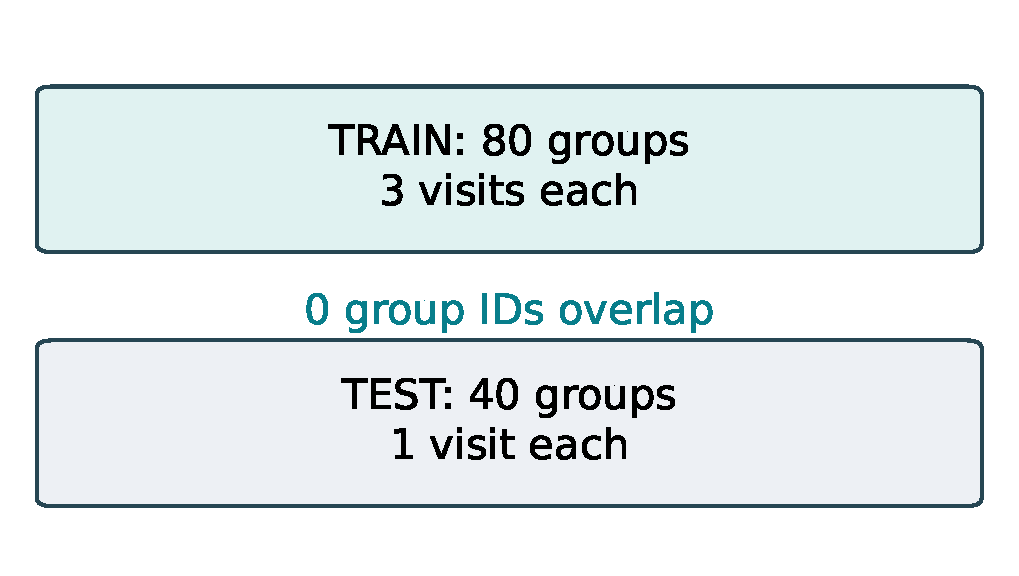
\includegraphics[width=.98\linewidth,height=.69\textheight,keepaspectratio]{presentation-figures/group-protocol-panel-1.pdf}\end{frame}
\renewcommand{\notestarget}{notes.pdf\#note-row-disjointness-and-group-disjointness}
\begin{frame}[label=slide-the-new-group-condition-panel-2]{Seen-group contamination}
\centering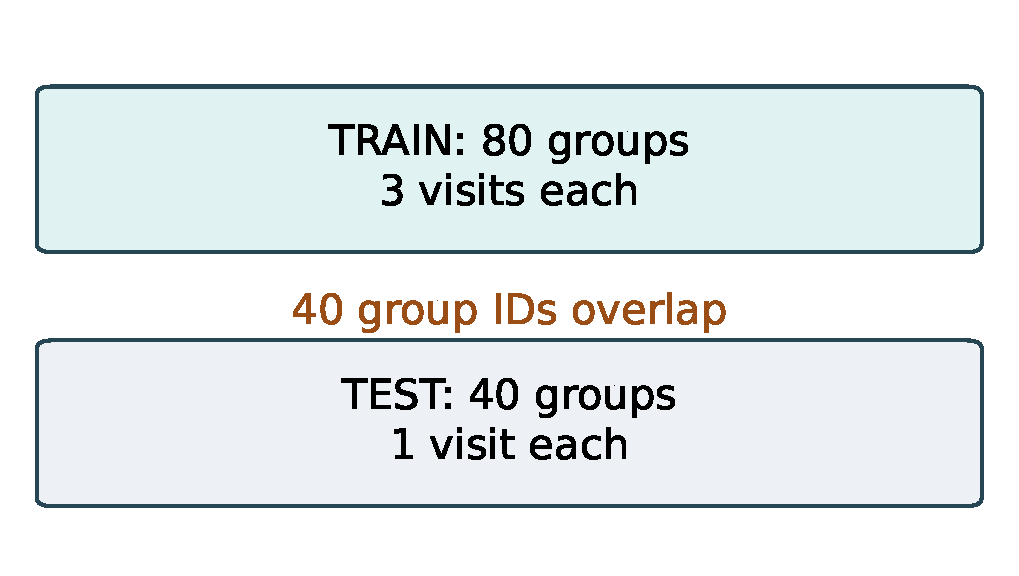
\includegraphics[width=.98\linewidth,height=.69\textheight,keepaspectratio]{presentation-figures/group-protocol-panel-2.pdf}\end{frame}
\renewcommand{\notestarget}{notes.pdf\#note-row-disjointness-and-group-disjointness}
\begin{frame}[t,fragile,label=slide-the-new-group-condition]{The new-group condition}
\[G_{train}\cap G_{test}=\varnothing.\]\pause{} Disjoint row indices do not imply this stronger condition.
\end{frame}
\renewcommand{\notestarget}{notes.pdf\#note-row-disjointness-and-group-disjointness}
\begin{frame}[t,fragile,label=slide-a-controlled-contamination]{A controlled contamination}
The same forty test rows are retained while training includes earlier repeats from their groups.\pause{} Training and test rows differ, but their fingerprints reveal shared identity.
\end{frame}
\renewcommand{\notestarget}{notes.pdf\#note-constant-logistic-and-nearest-neighbor-baselines}
\begin{frame}[t,fragile,label=slide-the-constant-baseline]{The constant baseline}
\[\widehat p=\frac1{N_{train}}\sum_i y_i.\]\pause{} Predict the training majority class, with the stated tie rule. No feature information enters.
\end{frame}
\renewcommand{\notestarget}{notes.pdf\#note-constant-logistic-and-nearest-neighbor-baselines}
\begin{frame}[t,fragile,label=slide-signal-only-logistic-prediction]{Signal-only logistic prediction}
\[p=\sigma(w\widetilde x_1+b).\]\pause{} This baseline uses the declared population signal without the random fingerprint coordinates.
\end{frame}
\renewcommand{\notestarget}{notes.pdf\#note-constant-logistic-and-nearest-neighbor-baselines}
\begin{frame}[t,fragile,label=slide-the-penalized-objective]{The penalized objective}
\[J=\frac1N\sum_i[\log(1+e^{z_i})-y_i z_i]+\frac\lambda2w^2.\]\pause{} The fixed penalty is selected without test outcomes.
\end{frame}
\renewcommand{\notestarget}{notes.pdf\#note-constant-logistic-and-nearest-neighbor-baselines}
\begin{frame}[t,fragile,label=slide-a-nearest-neighbor-rule]{A nearest-neighbor rule}
\[j_* =\arg\min_{j\in train}\|\widetilde x-\widetilde x_j\|^2,\qquad\widehat y=y_{j_*}.\]\pause{} Near-duplicate fingerprints make recognition easy.
\end{frame}
\renewcommand{\notestarget}{notes.pdf\#note-training-dependent-transformations}
\begin{frame}[t,fragile,label=slide-fit-the-coordinate-transformation-on-training-data]{Fit the coordinate transformation on training data}
\[\widetilde x_k=\frac{x_k-\mu_k^{train}}{s_k^{train}}.\]\pause{} Test cases reuse the same means and scales.
\end{frame}
\renewcommand{\notestarget}{notes.pdf\#note-training-dependent-transformations}
\begin{frame}[t,fragile,label=slide-standardization-defines-a-distance]{Standardization defines a distance}
\[\|\widetilde x-\widetilde x_j\|^2=\sum_k\frac{(x_k-x_{jk})^2}{(s_k^{train})^2}.\]\pause{} Refitting a scaler changes the nearest-neighbor metric.
\end{frame}
\renewcommand{\notestarget}{notes.pdf\#note-confusion-matrices-and-class-conditional-error}
\begin{frame}[t,fragile,label=slide-read-the-confusion-matrix]{Read the confusion matrix}
\[\begin{pmatrix}TN&FP\\FN&TP\end{pmatrix}.\]\pause{} Rows are true classes and columns are predicted classes. Each recall uses its true-class row total.
\end{frame}
\renewcommand{\notestarget}{notes.pdf\#note-confusion-matrices-and-class-conditional-error}
\begin{frame}[label=slide-balanced-accuracy-figure]{Accuracy on same 40 cases}
\centering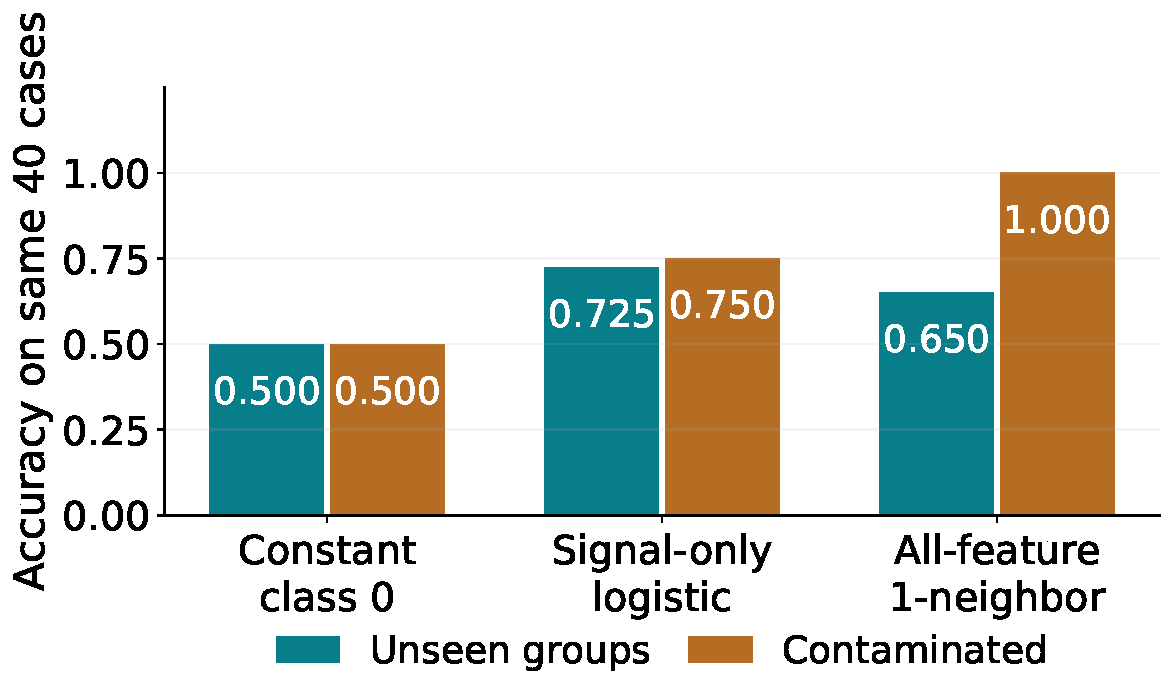
\includegraphics[width=.98\linewidth,height=.69\textheight,keepaspectratio]{presentation-figures/baseline-comparison-panel-1.pdf}\end{frame}
\renewcommand{\notestarget}{notes.pdf\#note-confusion-matrices-and-class-conditional-error}
\begin{frame}[t,fragile,label=slide-balanced-accuracy]{Balanced accuracy}
\[\mathrm{BA}=\frac12\left(\frac{TN}{TN+FP}+\frac{TP}{TP+FN}\right).\]\pause{} Both classes must be present.
\end{frame}
\renewcommand{\notestarget}{notes.pdf\#note-confusion-matrices-and-class-conditional-error}
\begin{frame}[t,fragile,label=slide-prevalence-weighted-accuracy]{Prevalence-weighted accuracy}
\[\mathrm{Accuracy}=(1-\pi)\mathrm{TNR}+\pi\mathrm{TPR}.\]\pause{} Balanced accuracy uses equal class weights instead of prevalence weights.
\end{frame}
\renewcommand{\notestarget}{notes.pdf\#note-the-scope-of-the-estimated-prediction-risk}
\begin{frame}[t,fragile,label=slide-recognition-is-not-new-group-prediction]{Recognition is not new-group prediction}
The contaminated nearest neighbor attains perfect accuracy on this constructed sample.\pause{} The result reflects access to the same group fingerprints, not perfect population discrimination.
\end{frame}
\renewcommand{\notestarget}{notes.pdf\#note-the-scope-of-the-estimated-prediction-risk}
\begin{frame}[t,fragile,label=slide-the-target-distribution-remains-an-assumption]{The target distribution remains an assumption}
Holding out people does not automatically hold out sites, calendar periods or acquisition devices.\pause{} Prediction-time availability and the group-generating distribution remain part of the statistical problem.
\end{frame}
\end{document}
